
\begin{figure}
\centering

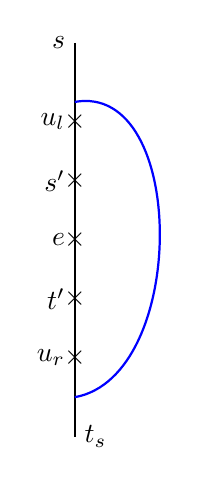
\begin{tikzpicture}[scale=1]

\coordinate (x) at (0,5);
\coordinate (y) at (0,0);
\coordinate (u) at (0,2.5);
\coordinate (ul) at (0,1);
\coordinate (ur) at (0,4);

\coordinate (x1) at (0,1.75);
\coordinate (y1) at (0,3.25);

\draw[thick](x)--(y);
\node[left] at (x){$s$};
\node[right] at (y){$t_{s}$};

\node[left] at (u){$e$};
\node at (u){$\times$};
\node[left] at (ul){$u_r$};
\node at (ul){$\times$};
\node[left] at (ur){$u_l$};
\node at (ur){$\times$};

\node[left] at (x1){$t'$};
\node at (x1){$\times$};
\node[left] at (y1){$s'$};
\node at (y1){$\times$};

\draw[thick,blue] (0,0.5) to[out=10,in=10] node[pos=0.2,
left]
{ } (0,4.25);
\end{tikzpicture}
\caption{The hardest part of the distance oracle, when the
replacement path neither passes through $u_l$ not $u_r$.}
\end{figure}
